\subsection{Funcionalidades do aplicativo}

Antes da contagem física dos produtos pelos auditores munidos de coletores, cabe ao administrador do inventário realizar sua devida configuração. Essa etapa compreende o registro do nome do inventário, definição do período de sua realização (data de início e término), indicação do depósito onde ocorrerá a contagem e a listagem dos produtos a serem inventariados.

\begin{figure}[!htb]
    \centering
    \subfigure[Tela de login.]{
        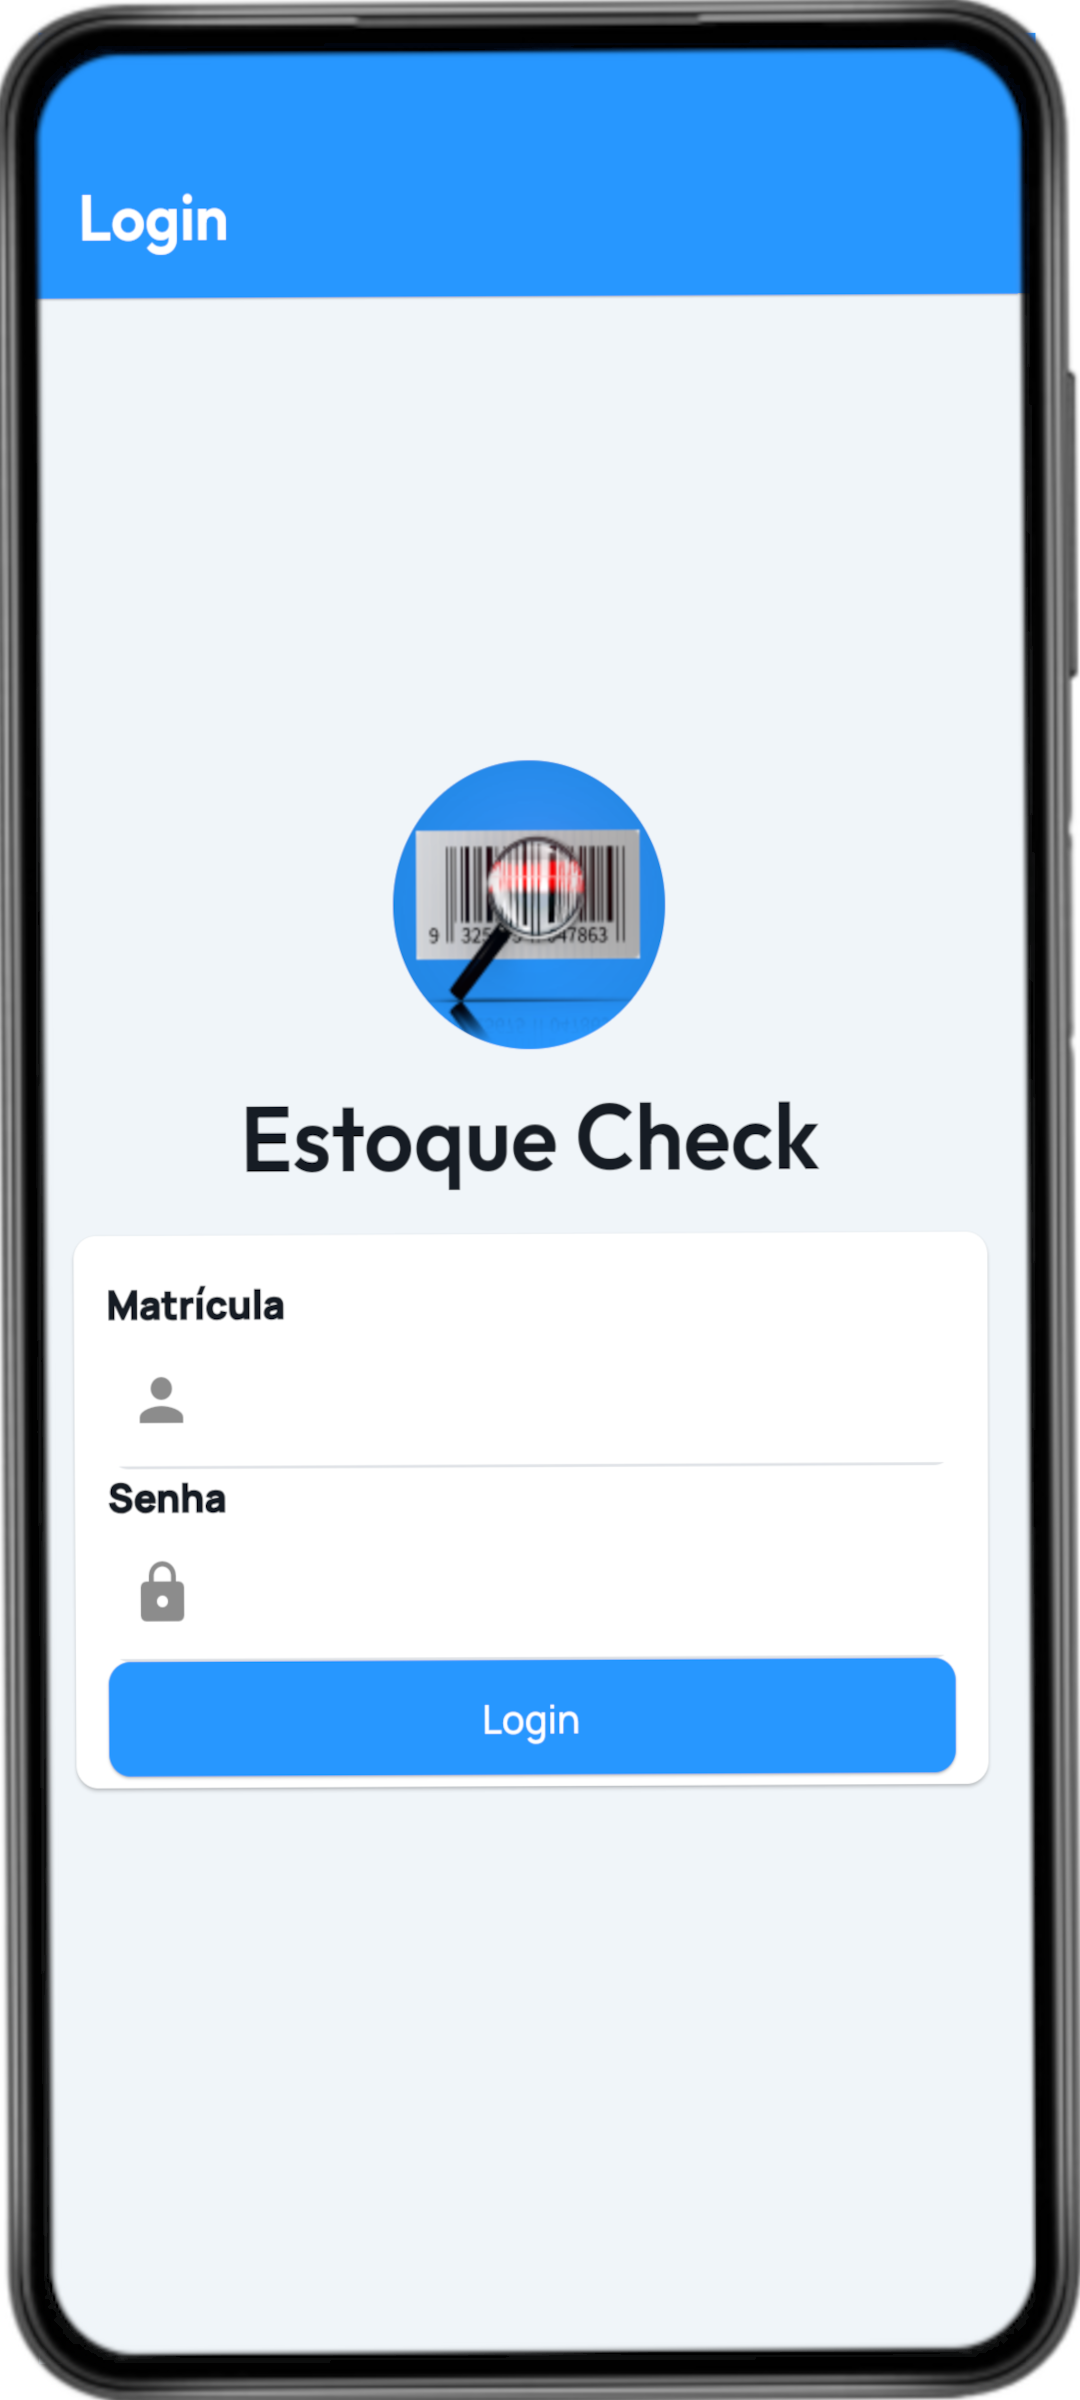
\includegraphics[width=0.15\textwidth]{imgs/login.png}
    }
    \quad
    \subfigure[Tela principal.]{
        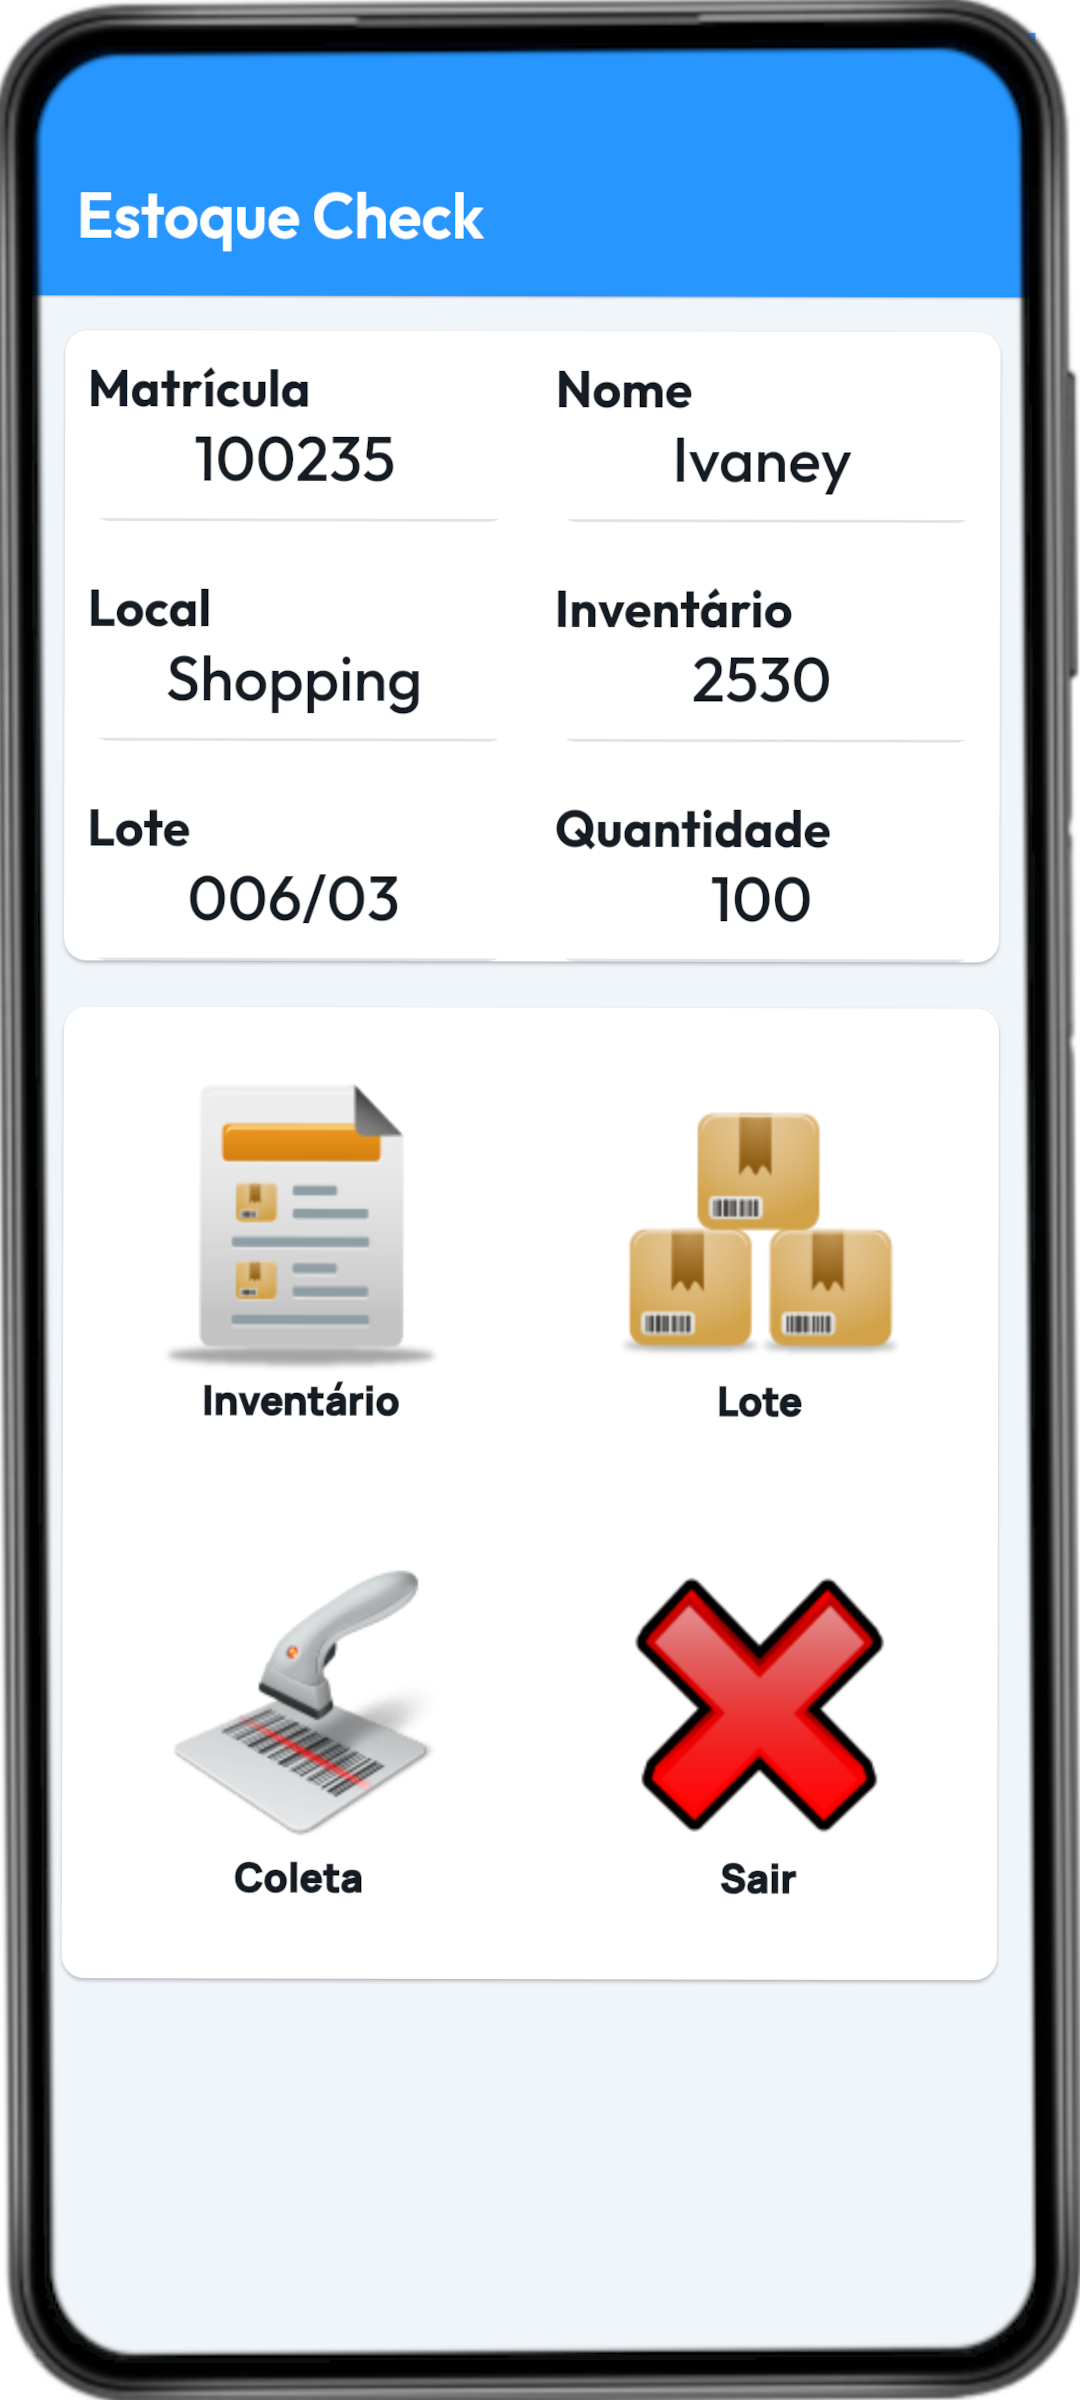
\includegraphics[width=0.15\textwidth]{imgs/homepage.png}
    }
    \quad
    \subfigure[Seleção de inventário.]{
        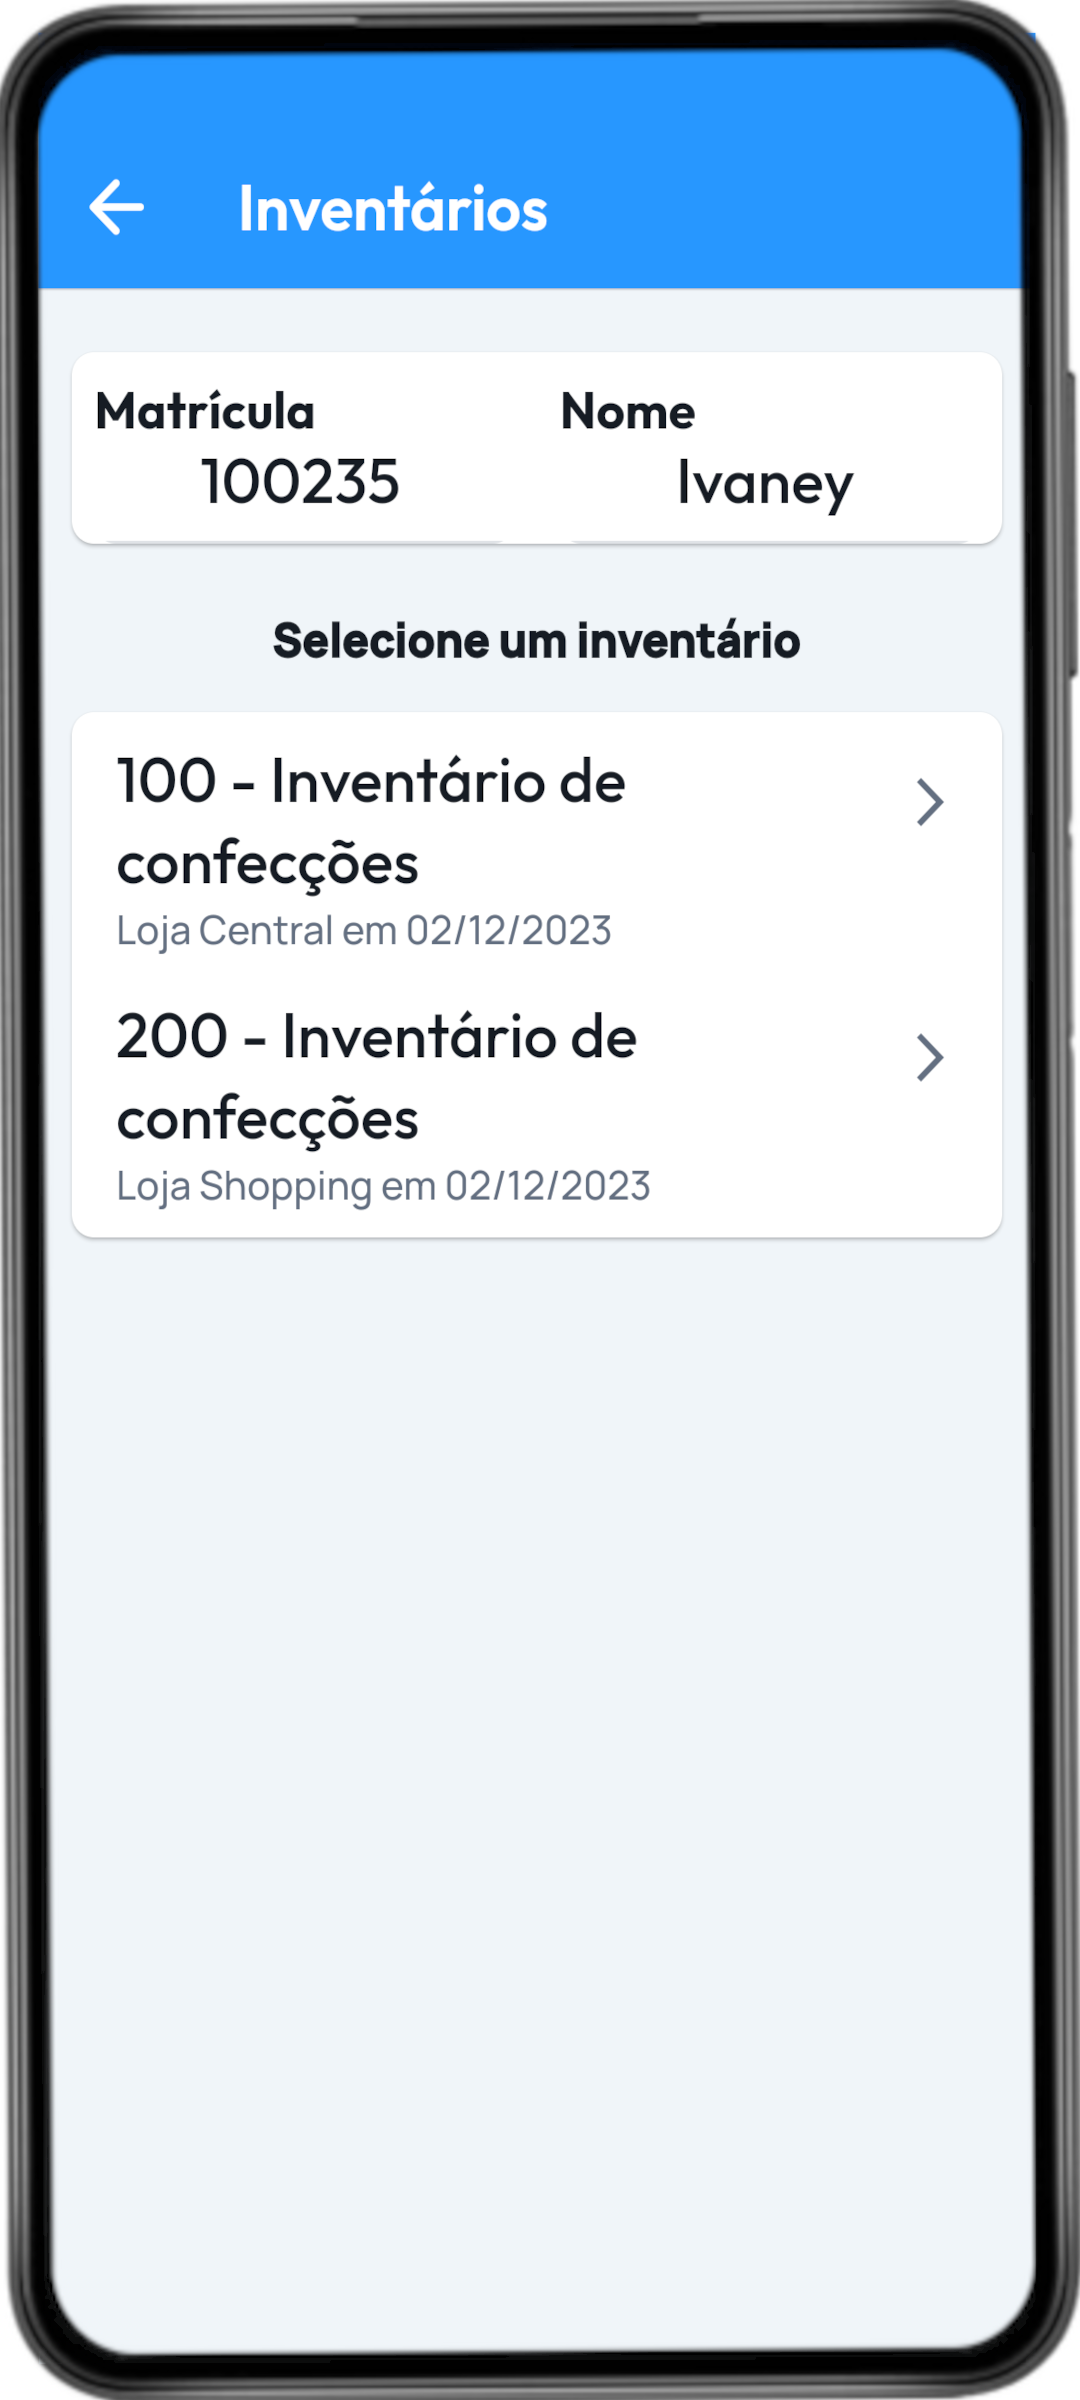
\includegraphics[width=0.15\textwidth]{imgs/inventario.png}
    }
    \quad
    \subfigure[Seleção de lote.]{
        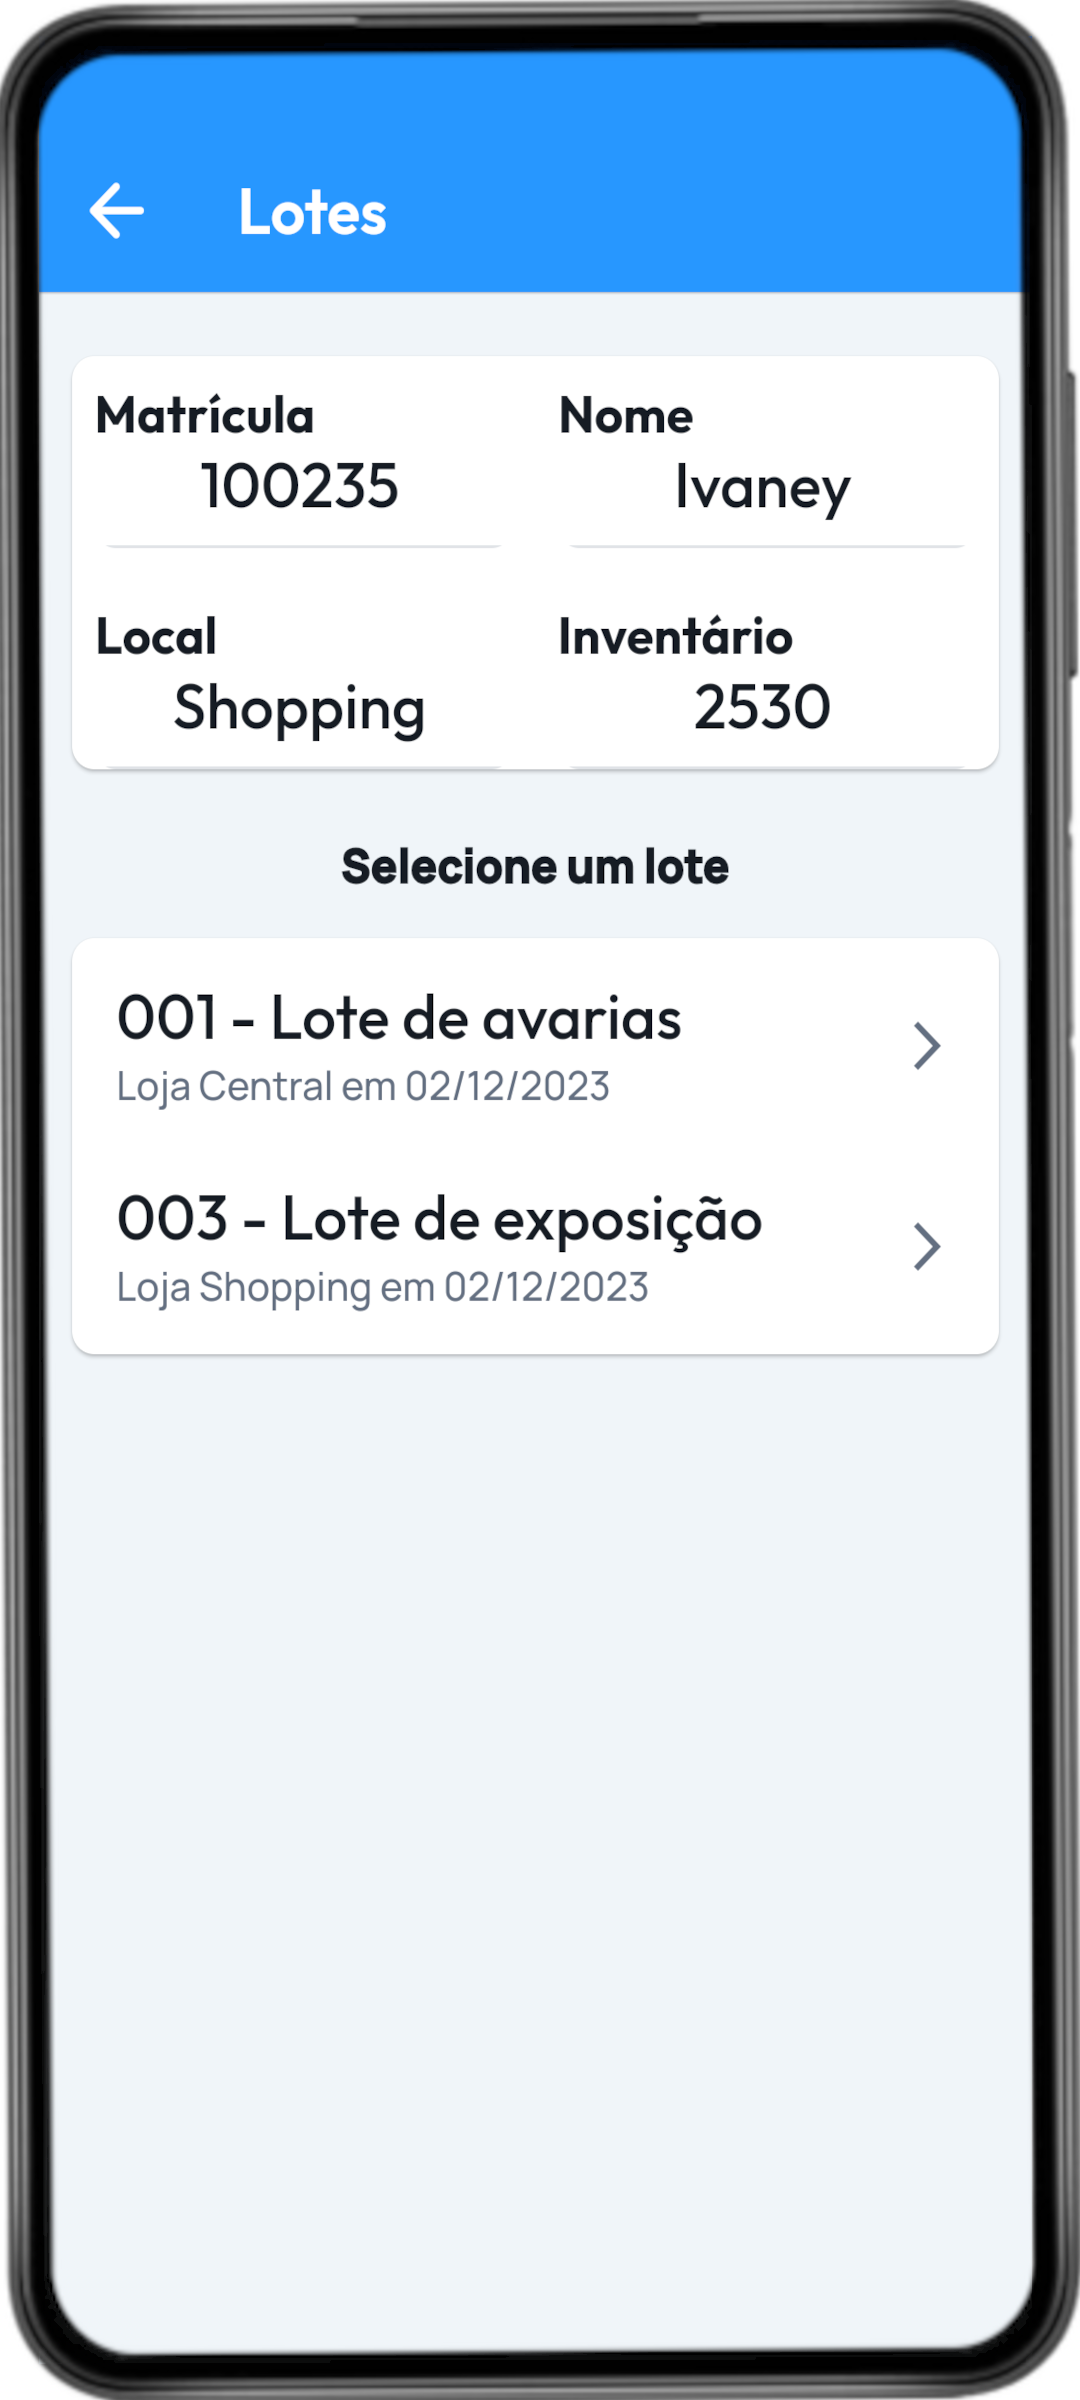
\includegraphics[width=0.15\textwidth]{imgs/lote.png}
    }
    \quad
    \subfigure[Coleta para contagem.]{
        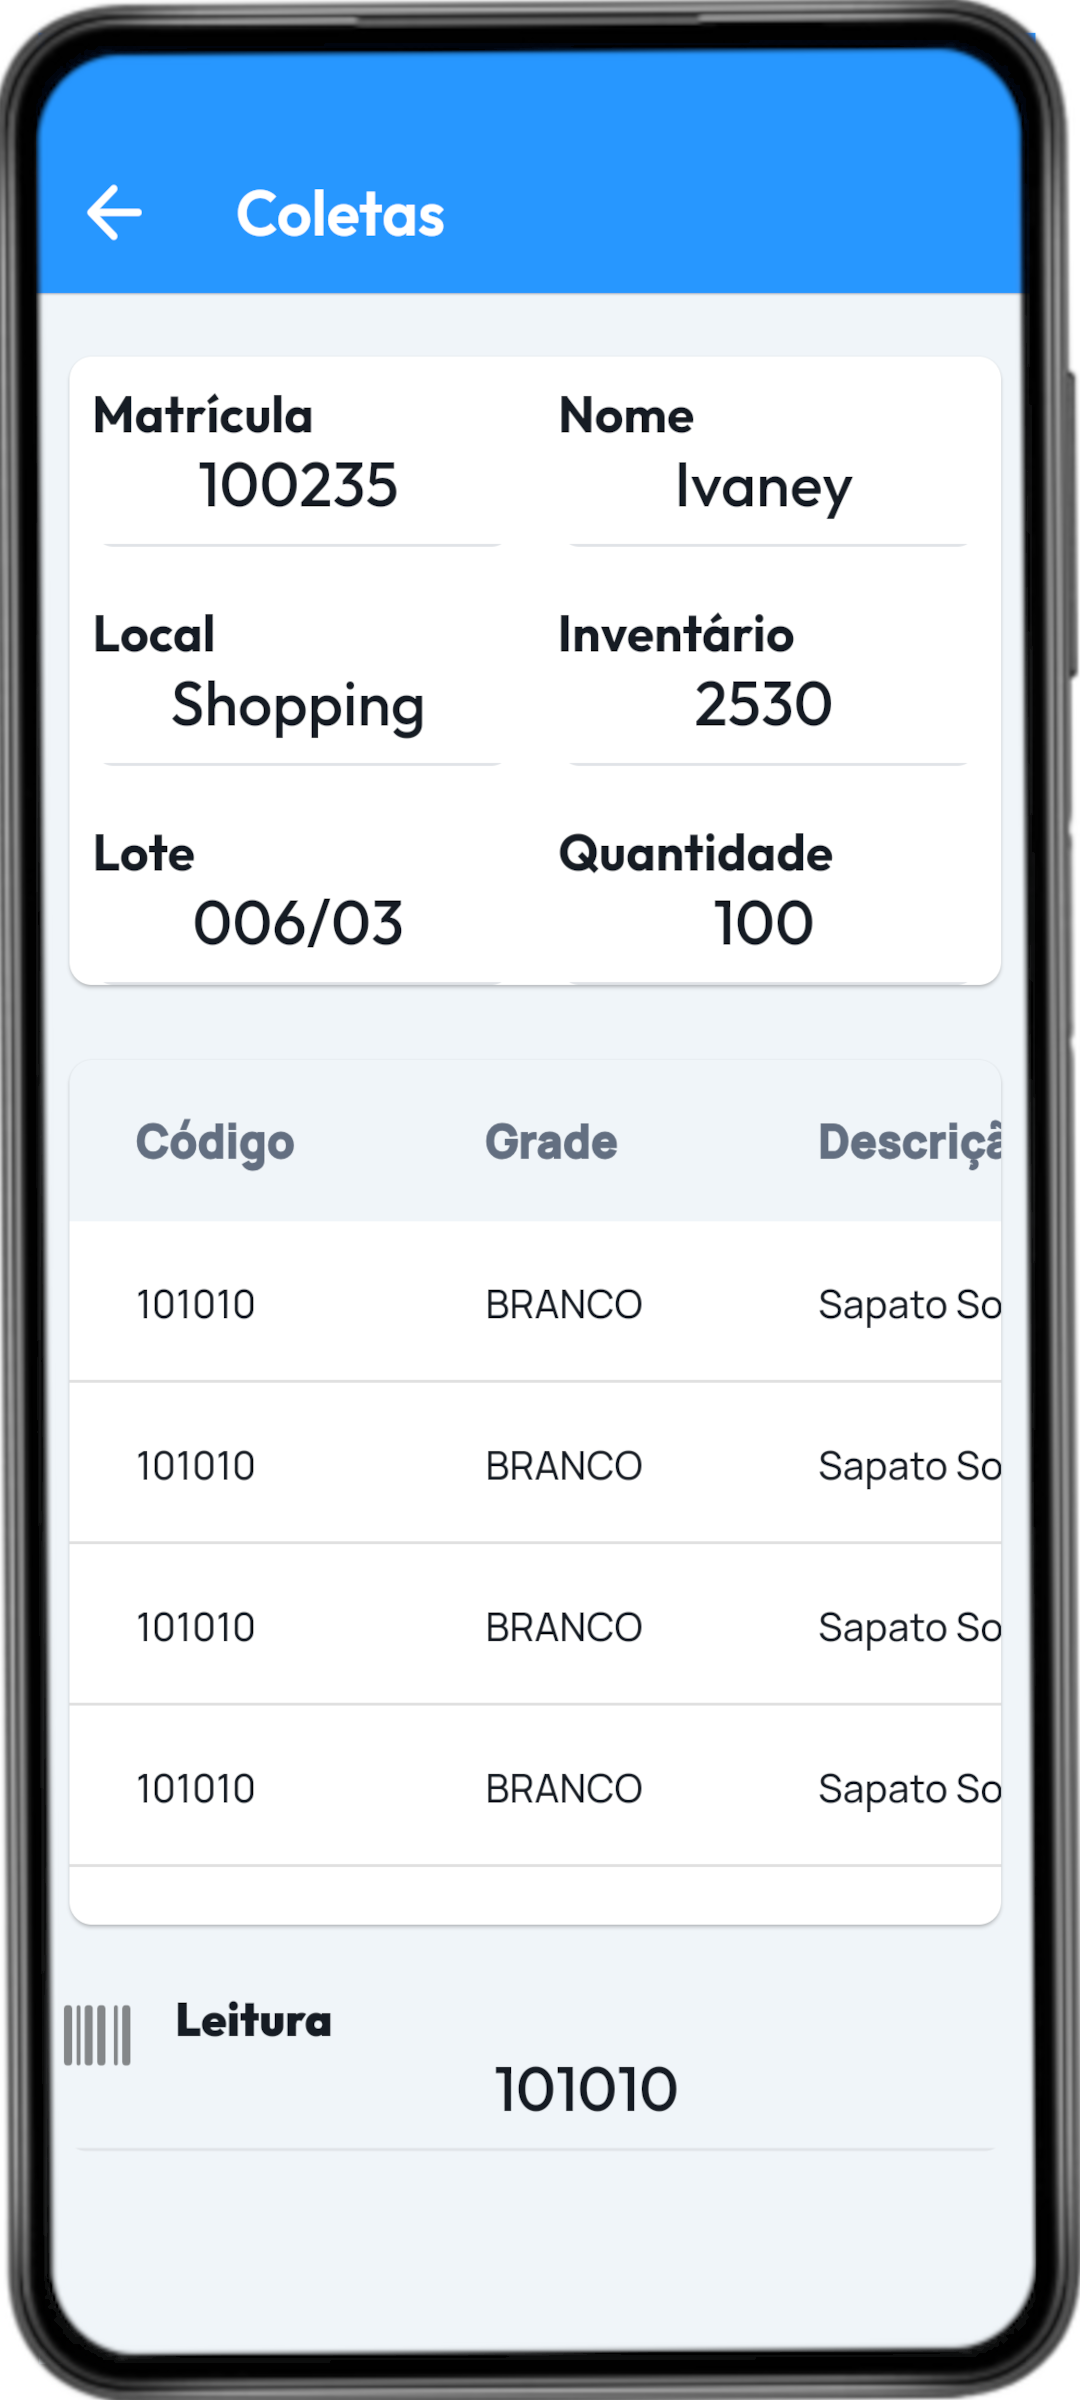
\includegraphics[width=0.15\textwidth]{imgs/coleta.png}
    }
    \caption{Layout de telas para o aplicativo}
    \label{fig:telas}
\end{figure}

A figura \ref{fig:telas} apresenta o layout das telas do aplicativo conforme descrito a seguir:

\begin{itemize}
    \item \textbf{Tela de Login}: Esta tela destina-se à autenticação do usuário no aplicativo. O usuário deve inserir seu nome de usuário e senha válidos, que correspondem às credenciais de acesso do sistema de gestão da empresa.

    \item \textbf{Tela Principal}: A tela principal apresenta ao usuário as opções para iniciar uma nova contagem de inventário ou retomar uma contagem já em andamento.

    \item \textbf{Seleção de Inventário}: Nesta tela, o usuário visualiza a lista de inventários disponíveis para contagem e seleciona aquele que deseja realizar o procedimento.

    \item \textbf{Seleção de Lote}: A tela de seleção de lote apresenta ao usuário a lista de lotes disponíveis dentro do inventário escolhido. O usuário deve selecionar o lote que deseja contar. Um lote é definido como um conjunto de produtos agrupados em um espaço físico específico, como um palete, uma gôndola ou uma estante. Cada lote é identificado por um código e um código de barras. O auditor pode selecionar o lote desejado lendo o código de barras com o coletor.

    \item \textbf{Coleta para Contagem}: Nesta tela, o usuário visualiza os produtos presentes no lote selecionado e registra a quantidade contada de cada item. Ao finalizar a contagem, os dados coletados são enviados ao sistema de gestão da empresa. Nesse momento, o status do lote é atualizado para “fechado”, podendo ser reaberto apenas pelo administrador do sistema.
\end{itemize}

Durante a contagem, o administrador monitora o progresso das contagens por meio de um dashboard e pode configurar alertas para serem enviados aos auditores, informando sobre a proximidade do término do inventário ou eventuais atrasos na contagem.

Após a conclusão da contagem, o administrador fecha o inventário. Os dados são validados por meio de uma análise estatística e, em seguida, processados para realizar ajustes gerenciais e fiscais do estoque.

\subsection{Aplicativos semelhantes}

A tabela \ref{tab:comparativos} uma comparação entre os aplicativos IS Collector, KCollector e Stock e Inventário Simples, que são aplicativos de contagem de inventário disponíveis na loja de aplicativos do Google. A análise abrange suas principais funcionalidades.

\begin{table}[!htb]
    \centering
    \caption{Funcionalidades dos aplicativos semelhantes.}
    \label{tab:comparativos}
    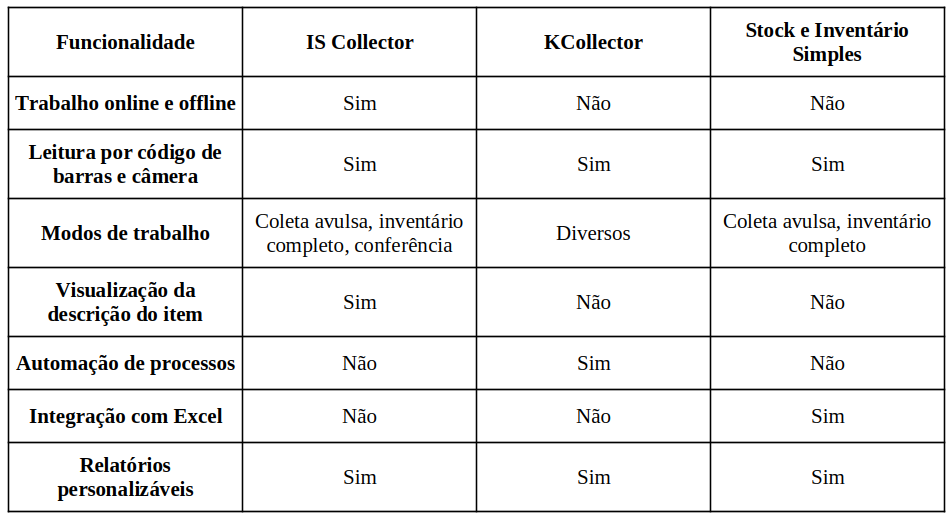
\includegraphics[width=1.0\textwidth]{tables/comparativo.png}
    %Fonte: \cite{googleplay}.
\end{table}

O IS Collector se destaca pela flexibilidade e abrangência de funções, ideal para empresas que exigem um alto nível de controle e automação no processo de inventário. O KCollector é a opção ideal para quem busca uma solução acessível e prática, que transforma o celular em um coletor eficiente. Já o Stock e Inventário Simples se destaca pela facilidade de uso e pelo gerenciamento completo do estoque, sendo uma ótima opção para iniciantes e pequenos negócios.

% Colocar aqui um parágrafo comparando o aplicativo do trabalho com os aplicativos pesquisados
O aplicativo do presente trabalho se destaca pela integração com o sistema de gestão da empresa, garantindo a consistência e a atualização em tempo real dos dados de estoque. Além disso, a interface intuitiva e as funcionalidades customizáveis proporcionam uma experiência de usuário eficiente e adaptável às necessidades específicas de cada empresa. A integração com tecnologias avançadas, como leitura de códigos de barras e alerta automatizados, eleva a eficácia do aplicativo, tornando-o uma solução completa e moderna para o controle de inventário.
